% This file was adapted from ICLR2022_conference.tex example provided for the ICLR conference
\documentclass{article} % For LaTeX2e
\usepackage{conference,times}
\usepackage{easyReview}
\usepackage{algorithm}
\usepackage{algorithmic}

% Optional math commands from https://github.com/goodfeli/dlbook_notation.
\input{math_commands.tex}

\usepackage{amsthm,amssymb}

\newtheorem{theorem}{Theorem}[section]
\newtheorem{corollary}{Corollary}[theorem]
\newtheorem{lemma}[theorem]{Lemma}
\newtheorem{definition}[theorem]{Definition}

% Please leave these options as they are
\usepackage{hyperref}
\hypersetup{
    colorlinks=true,
    linkcolor=red,
    filecolor=magenta,
    urlcolor=blue,
    citecolor=purple,
    pdftitle={Curiosity-Conditioned Goal-Optimal Reinforcement Learning: Formal Envelopes and Stability Diagnostics},
    pdfpagemode=FullScreen,
    }




\title{Curiosity-Conditioned Goal-Optimal Reinforcement Learning}

\author{Anonymous Authors \\
Affiliation withheld for double-blind review \\
\texttt{anonymous@anonymous.edu}}

\begin{document}


\maketitle

\begin{abstract}
Goal-conditioned reinforcement learning often faces a practical tension: intrinsic novelty bonuses accelerate discovery in sparse and deceptive environments, but poorly controlled intrinsic coupling can distort the asymptotic objective. This paper introduces Curiosity-Conditioned Goal-Optimal Reinforcement Learning (CCGO-RL), a dual-value framework that treats curiosity as a controlled exploration mechanism inside a goal-conditioned control loop rather than as a permanent co-objective. The method combines an extrinsic value stream, an intrinsic value stream, confidence-bounded intrinsic annealing, and uncertainty-gated contrastive coupling. We formalize the setting with explicit decision variables (policy and scheduler), a measurable feasible scheduler set, and an optimality criterion based on extrinsic return. We prove a perturbation bound between mixed and extrinsic objectives and an extrinsic suboptimality envelope for mixed-objective optimization, and we derive a gate-sensitivity and conditional variance-increment bound for uncertainty-gated contrastive coupling. Empirically, synthetic benchmark suites covering sparse navigation, deceptive mazes, and goal-conditioned control show improved return-speed trade-offs and lower critic instability against strong baselines, with quantitative checks tied to theorem assumptions. The empirical gains are strongest for exploration efficiency and variance control, while one symbolic limit-corollary check remains mismatched, which narrows the interpretation of the asymptotic claim to the audited admissible schedule regime.
\end{abstract}


\section{Introduction}
\label{sec:introduction}

Goal-conditioned reinforcement learning (RL) is increasingly used in robotics, navigation, and long-horizon control because explicit goals provide a clean interface between task specification and policy optimization \citep{ref_universal_value_function_approximators_2015, arxiv1707_01495, arxiv2206_07568}. However, sparse and deceptive rewards continue to expose a core failure mode: policies that optimize only extrinsic return may fail to discover useful behaviors within realistic training horizons, while strong intrinsic bonuses can improve discovery yet bias the long-run objective \citep{arxiv1606_01868, arxiv1705_05363, arxiv1810_12894, arxiv2002_06038}. This tension is now visible across both classic exploration methods and newer adaptive curricula, including directed exploration and representation-heavy goal-space methods \citep{arxiv2003_13350, arxiv2505_19850, arxiv2603_14887, arxiv2603_02104, arxiv2602_24081}.

The design problem is therefore not simply ``add curiosity'' versus ``remove curiosity''; it is an optimization design problem with coupled objectives, uncertainty, and stability constraints. If intrinsic coupling is treated as a fixed coefficient, one often gets early exploration gains but fragile asymptotic behavior. If intrinsic coupling is aggressively annealed without uncertainty awareness, one can preserve asymptotic return but lose robustness under non-stationary replay distributions. At the same time, practical literature comparisons are often confounded by protocol inconsistencies in seed counts, runtime normalization, and reporting granularity \citep{arxiv1912_01588, arxiv2004_07219, arxiv2405_19548}. The result is a gap between algorithmic intuition and auditable evidence.

This paper investigates whether a confidence-bounded and uncertainty-gated coupling law can preserve extrinsic optimality envelopes while retaining practical exploration gains. Our scope is hybrid: we derive formal bounds and then tie each major claim to executed diagnostics, rather than presenting proof-only claims or benchmark-only claims. The problem framing follows the selected goal-conditioned path from upstream synthesis: dual-value coupling is treated as adapted prior art, while the scheduler feasible set, envelope statements, and theorem-aligned diagnostics are manuscript-specific formalizations.

Our contributions are:
\begin{itemize}
  \item We define a goal-conditioned mixed-objective control setting with explicit decision variables, feasible scheduler set, and extrinsic optimality criterion that makes the policy--scheduler trade-off mathematically explicit.
  \item We prove a perturbation bound and an extrinsic suboptimality envelope for confidence-bounded intrinsic annealing, including conditions under which mixed-objective optimization converges back to extrinsic-optimal behavior.
  \item We introduce and analyze uncertainty-gated contrastive coupling with a Lipschitz gate-sensitivity result and a conditional variance-increment bound that links representation coupling to critic stability.
  \item We provide theorem-aligned empirical evidence on sparse/deceptive and goal-conditioned suites, including non-inferiority analyses, counterexample stress tests, and explicit caveats where symbolic checks and empirical audits diverge.
\end{itemize}

The broader relevance is that the same coupling logic appears in multi-objective control beyond RL, including reward shaping, uncertainty-aware planning, and adaptive safety margins; therefore, clarifying objective perturbation versus asymptotic recovery has cross-domain implications for any system that uses temporary auxiliary signals to accelerate optimization.

\section{Background and Problem Setting}
\label{sec:problem}

\subsection{Control Setting and Notation}

We consider a discounted goal-conditioned Markov decision process with state space $\mathcal{S}$, action space $\mathcal{A}$, goal space $\mathcal{G}$, transition kernel $P(s'\mid s,a)$, and discount factor $\gamma\in(0,1)$. A stochastic goal-conditioned policy is denoted $\pi_\theta(a\mid s,g)$, where $\theta$ are learnable parameters. This setting follows the UVFA/HER lineage, where goals parameterize value and policy functions \citep{ref_universal_value_function_approximators_2015, arxiv1707_01495, arxiv1912_06088}.

The extrinsic reward is $r_t^e$, and an intrinsic exploration signal is $r_t^i$. Mixed-reward optimization with additive coupling has substantial precedent in curiosity and intrinsic motivation literature \citep{arxiv1703_01310, arxiv1810_12894, arxiv1705_05363, arxiv2602_24081}. In this work, we adopt that coupling form but define a constrained scheduler class and theorem-audited envelopes that are specific to this manuscript.

\subsection{Objective, Decision Variables, and Feasible Set}

We define the extrinsic objective and mixed objective as
\begin{equation}
\label{eq:Je}
J_e(\pi)=\mathbb{E}_{\pi}\!\left[\sum_{t=0}^{\infty}\gamma^t r_t^e\right],
\end{equation}
\begin{equation}
\label{eq:Jmix}
J_{\mathrm{mix}}(\pi,\beta)=\mathbb{E}_{\pi}\!\left[\sum_{t=0}^{\infty}\gamma^t\left(r_t^e+\beta_t r_t^i\right)\right].
\end{equation}
Here $\beta_t\in[0,\beta_{\max}]$ is an adaptive intrinsic weight. We define the feasible scheduler set in this work as
\begin{equation}
\label{eq:feasibleB}
\mathcal{B}=\left\{\beta:\beta_t\in[0,\beta_{\max}],\ \beta_t\ \mathcal{F}_t\text{-measurable},\ M_\beta:=\sum_{t=0}^{\infty}\gamma^t\mathbb{E}[\beta_t]<\infty\right\},
\end{equation}
where $\mathcal{F}_t$ is the filtration generated by non-privileged trajectory history. The decision variables are $(\pi,\beta)\in\Pi\times\mathcal{B}$. The primary optimality criterion is extrinsic:
\begin{equation}
\label{eq:pi_star}
\pi^\star\in\arg\max_{\pi\in\Pi}J_e(\pi).
\end{equation}
The mixed objective is used as an exploration-accelerating proxy, not the terminal objective.

\subsection{Assumptions and Scope of Claims}

We assume bounded rewards $|r_t^e|\le R_e$ and $|r_t^i|\le R_i$, finite discounted intrinsic mass $M_\beta<\infty$, and non-privileged scheduler observability. These assumptions are standard in spirit for bounded-return control arguments but their specific packaging in \eqref{eq:feasibleB} is manuscript-defined. We also assume standard off-policy critic stability scaffolds adapted from actor-critic practice \citep{arxiv1509_02971, arxiv1707_06347, arxiv1802_09477, arxiv1801_01290}. The derived claims are therefore conditional guarantees on this admissible regime, not global guarantees over arbitrary scheduler dynamics.

\section{Related Work and Novelty Boundary}
\label{sec:related}

\subsection{Goal-Conditioned RL and Replay-Based Generalization}

Goal-conditioned learning evolved from UVFA-style conditioning to HER-style relabeling and then to representation-aware contrastive variants \citep{ref_universal_value_function_approximators_2015, arxiv1707_01495, arxiv1903_03698, arxiv1912_06088, arxiv2206_07568}. HER remains a robust baseline in sparse settings because relabeling partially repairs reward sparsity without changing environment dynamics. Contrastive and augmentation methods (for example CRL-style and ViSA/ACDC families) often improve sample efficiency but can introduce sensitivity to encoder quality, negative sampling, and coupling hyperparameters \citep{arxiv2206_07568, arxiv2603_14887, arxiv2603_02104, arxiv2603_29533}.

The consensus from our acquired corpus is that explicit goal structure plus replay is reliable, yet the superiority of representation-heavy alternatives is regime-dependent and protocol-sensitive. This motivates a design that keeps a replay-compatible backbone while using uncertainty-aware coupling to bound instability.

\subsection{Intrinsic Motivation, Exploration Pressure, and Failure Modes}

Count-based and pseudo-count methods established principled novelty incentives in sparse settings \citep{arxiv1606_01868}. Prediction-error families (ICM, RND) made novelty scaling practical, but highlighted non-stationarity and reward-channel interference \citep{arxiv1703_01310, arxiv1810_12894}. Directed exploration systems, including episodic-lifelong hybrids and hard-exploration pipelines, demonstrated strong discovery behavior at the cost of complexity and weaker comparability across protocols \citep{arxiv2002_06038, arxiv2003_13350, arxiv1901_10995}. Newer adaptive curricula and entropy-coverage variants further improved early discovery, yet many still under-specify how intrinsic influence is controlled near convergence \citep{arxiv2412_03800, arxiv2505_19850, arxiv2509_03790, arxiv2602_24081}.

The key contradiction is therefore not whether curiosity helps; it is whether curiosity can help without distorting asymptotic task optimality. Existing papers frequently answer one side but leave the other under-specified.

\subsection{Stability, Comparability, and Benchmark Discipline}

Optimization backbones from DDPG/PPO/TD3/SAC and auxiliary-task systems such as UNREAL provide practical stability scaffolds, but they do not by themselves resolve objective-coupling drift \citep{arxiv1509_02971, arxiv1511_05952, arxiv1707_06347, arxiv1802_09477, arxiv1801_01290, arxiv1611_05397}. Benchmark infrastructure (Gymnasium, MiniGrid, Procgen, D4RL, and tooling suites such as RLeXplore) improves reproducibility, yet literature still suffers from inconsistent seed discipline and unequal runtime envelopes \citep{ref_gymnasium_2023, ref_minigrid_2023, arxiv1912_01588, arxiv2004_07219, arxiv2006_12983, arxiv2405_19548}.

Our novelty boundary follows directly from this synthesis. Mixed-reward coupling, goal relabeling, and contrastive value components are adapted from prior work; what is new here is the explicit scheduler feasible set, theorem-level envelopes with auditable assumptions, and a claim-evidence structure that forces each formal statement to terminate in diagnostics rather than implicit plausibility.

\section{Method: Curiosity-Conditioned Goal-Optimal RL}
\label{sec:method}

\subsection{Dual-Value Architecture and Confidence-Bounded Scheduling}

CCGO-RL maintains two value channels: an extrinsic channel $Q_e(s,a,g)$ and an intrinsic channel $Q_i(s,a,g)$, with a mixed target used only for training acceleration. The policy update remains anchored to extrinsic return, while the intrinsic channel modulates exploration through $\beta_t$. We instantiate a confidence signal $c_t\in[0,1]$ based on goal-progress reliability and a calibrated uncertainty proxy $u_t\in[0,1]$ derived from critic disagreement and prediction variance. The scheduler is
\begin{equation}
\label{eq:beta_scheduler}
\beta_t = \beta_{\max}\,\sigma\!\left(\kappa_c(\tau_c-c_t)\right)\,\sigma\!\left(\kappa_u(u_t-\tau_u)\right),
\end{equation}
where $\sigma(\cdot)$ is the logistic function. This form preserves boundedness by construction and decreases intrinsic influence as confidence grows unless uncertainty remains high.

The first factor in \eqref{eq:beta_scheduler} is the confidence-bounded annealing mechanism; the second is a stability guard that avoids prematurely collapsing intrinsic support when epistemic uncertainty is still high. This decomposition was selected because literature contradictions show that fixed coupling over-drives curiosity late in training, while purely confidence-only annealing can under-explore under estimator noise \citep{arxiv1810_12894, arxiv2002_06038, arxiv2602_24081}.

\subsection{Uncertainty-Gated Contrastive Coupling}

To connect replay robustness with representation power, we use a HER-compatible backbone and a gated contrastive residual:
\begin{equation}
\label{eq:qmix}
Q_{\mathrm{mix}}(s,a,g)=Q_{\mathrm{HER}}(s,a,g)+\lambda_t Q_{\mathrm{CTR}}(s,a,g),
\end{equation}
\begin{equation}
\label{eq:lambda}
\lambda_t = \sigma\!\left(\kappa(u_t-\tau)\right)\in[0,1].
\end{equation}
The coupling form in \eqref{eq:qmix} is adapted from goal-conditioned contrastive lineages \citep{arxiv2206_07568, arxiv2603_14887}, while the gate in \eqref{eq:lambda} and its theorem-audited sensitivity bound are manuscript-specific. For temporal-difference updates we use
\begin{equation}
\label{eq:ytarget}
Y_t=r_t^e+\gamma\left(Q_{\mathrm{HER},t+1}+\lambda_t\left(Q_{\mathrm{CTR},t+1}^{\star}+\xi_t\right)\right),
\end{equation}
where $\xi_t$ denotes contrastive target noise with conditional mean zero and bounded variance envelope.

\subsection{Policy Update Logic and Training Procedure}

The optimization logic is intentionally simple: critic learning uses mixed targets for exploration efficiency; policy improvement is evaluated under extrinsic return and regularized by stability diagnostics. This prevents the intrinsic channel from redefining task optimality while preserving practical exploration benefit in early and mid training. The resulting procedure remains compatible with off-policy actor-critic pipelines and replay infrastructures \citep{arxiv1707_01495, arxiv1801_01290, arxiv2206_07568}.

\begin{algorithm}[t]
\caption{CCGO-RL Training Loop}
\label{alg:ccgo}
\begin{algorithmic}[1]
\STATE Initialize policy $\pi_\theta$, extrinsic critic $Q_e$, intrinsic critic $Q_i$, target networks, and replay buffer $\mathcal{R}$.
\FOR{each environment step}
  \STATE Collect transition $(s_t,a_t,r_t^e,s_{t+1},g_t)$ and append to $\mathcal{R}$ with goal-conditioned relabel candidates.
  \STATE Estimate confidence $c_t$ and uncertainty proxy $u_t$ from critic statistics and prediction residuals.
  \STATE Compute intrinsic weight $\beta_t$ using \eqref{eq:beta_scheduler} and contrastive gate $\lambda_t$ using \eqref{eq:lambda}.
  \STATE Form mixed critic target with \eqref{eq:ytarget}; update $Q_e,Q_i$ (and $Q_{\mathrm{CTR}}$ when active) by mini-batch TD minimization.
  \STATE Update policy parameters $\theta$ against extrinsic objective proxy while monitoring critic-drift and reward-channel dominance diagnostics.
  \STATE Soft-update target networks; log $\widehat{M}_\beta$, variance diagnostics, and bound-residual statistics.
\ENDFOR
\STATE Return policy checkpoint selected by extrinsic validation performance under fixed evaluation protocol.
\end{algorithmic}
\end{algorithm}

\section{Formal Analysis}
\label{sec:theory}

This section formalizes what is inherited and what is new. The mixed reward form in \eqref{eq:Jmix} is adapted from prior intrinsic-extrinsic coupling literature \citep{arxiv1705_05363, arxiv1810_12894, arxiv2602_24081}. In contrast, the feasible scheduler class \eqref{eq:feasibleB}, the envelope structure below, and the uncertainty-gated variance statement are defined in this work.

\begin{theorem}[Perturbation Bound]
\label{thm:perturbation}
Assume $|r_t^i|\le R_i$ and $\beta\in\mathcal{B}$. For any policy $\pi\in\Pi$,
\begin{equation}
\label{eq:perturbation_bound}
\left|J_{\mathrm{mix}}(\pi,\beta)-J_e(\pi)\right|\le R_i M_\beta.
\end{equation}
\end{theorem}
\begin{proof}
From \eqref{eq:Je} and \eqref{eq:Jmix},
\[
J_{\mathrm{mix}}(\pi,\beta)-J_e(\pi)=\mathbb{E}_{\pi}\!\left[\sum_{t=0}^{\infty}\gamma^t\beta_t r_t^i\right].
\]
Applying absolute value and triangle inequality gives
\[
\left|J_{\mathrm{mix}}-J_e\right|\le \sum_{t=0}^{\infty}\gamma^t\mathbb{E}[\beta_t|r_t^i|]
\le \sum_{t=0}^{\infty}\gamma^t\mathbb{E}[\beta_t R_i]
=R_i\sum_{t=0}^{\infty}\gamma^t\mathbb{E}[\beta_t]=R_iM_\beta,
\]
where finiteness follows from $\beta\in\mathcal{B}$. This proves \eqref{eq:perturbation_bound}.
\end{proof}

\begin{theorem}[Extrinsic Suboptimality Envelope]
\label{thm:gap}
Let $\hat\pi$ be $\varepsilon$-optimal for $J_{\mathrm{mix}}(\cdot,\beta)$ over $\Pi$, i.e.,
$\sup_{\pi\in\Pi}J_{\mathrm{mix}}(\pi,\beta)-J_{\mathrm{mix}}(\hat\pi,\beta)\le\varepsilon$.
Then
\begin{equation}
\label{eq:gap_envelope}
J_e(\pi^\star)-J_e(\hat\pi)\le 2R_iM_\beta+\varepsilon.
\end{equation}
\end{theorem}
\begin{proof}
By \eqref{eq:perturbation_bound}, for any $\pi$,
$J_e(\pi)\le J_{\mathrm{mix}}(\pi,\beta)+R_iM_\beta$ and
$J_{\mathrm{mix}}(\pi,\beta)\le J_e(\pi)+R_iM_\beta$.
Apply the first inequality to $\pi^\star$:
\[
J_e(\pi^\star)\le J_{\mathrm{mix}}(\pi^\star,\beta)+R_iM_\beta
\le \sup_{\pi\in\Pi}J_{\mathrm{mix}}(\pi,\beta)+R_iM_\beta.
\]
Using $\varepsilon$-optimality of $\hat\pi$,
\[
J_e(\pi^\star)\le J_{\mathrm{mix}}(\hat\pi,\beta)+\varepsilon+R_iM_\beta.
\]
Apply the second inequality to $\hat\pi$:
\[
J_{\mathrm{mix}}(\hat\pi,\beta)\le J_e(\hat\pi)+R_iM_\beta.
\]
Combining yields
\[
J_e(\pi^\star)\le J_e(\hat\pi)+2R_iM_\beta+\varepsilon,
\]
which is equivalent to \eqref{eq:gap_envelope}.
\end{proof}

\begin{lemma}[Gate Sensitivity]
\label{lem:lipschitz}
Let $\lambda(u)=\sigma(\kappa(u-\tau))$ for $u\in[0,1]$. Then for all $u,v\in[0,1]$,
\begin{equation}
\label{eq:lipschitz}
|\lambda(u)-\lambda(v)|\le \frac{\kappa}{4}|u-v|.
\end{equation}
\end{lemma}
\begin{proof}
Differentiate $\lambda$: $\lambda'(u)=\kappa\sigma(z)(1-\sigma(z))$ with $z=\kappa(u-\tau)$. Since $x(1-x)\le 1/4$ for all $x\in[0,1]$, we have $|\lambda'(u)|\le\kappa/4$. The mean-value theorem gives
$|\lambda(u)-\lambda(v)|\le\sup_{w\in[u,v]}|\lambda'(w)|\,|u-v|\le(\kappa/4)|u-v|$.
\end{proof}

\begin{theorem}[Conditional Variance Increment]
\label{thm:variance}
Assume $\mathbb{E}[\xi_t\mid\mathcal{F}_t]=0$ and
$\mathrm{Var}(\xi_t\mid\mathcal{F}_t)\le \sigma^2_{\xi}(u_t)\le\sigma^2_{\xi,\max}$.
Let $Y_t$ be defined by \eqref{eq:ytarget}. Then
\begin{equation}
\label{eq:variance_increment}
\Delta\mathrm{Var}_t:=\mathrm{Var}(Y_t\mid\mathcal{F}_t)-\mathrm{Var}(Y_t\mid\mathcal{F}_t,\xi_t\equiv0)
\le \gamma^2\lambda_t^2\sigma^2_{\xi}(u_t)
\le \gamma^2\sigma^2_{\xi,\max}\lambda_t^2.
\end{equation}
\end{theorem}
\begin{proof}
Let $\widetilde{Y}_t$ be $Y_t$ with $\xi_t\equiv0$. By \eqref{eq:ytarget},
$Y_t=\widetilde{Y}_t+\gamma\lambda_t\xi_t$.
Conditioned on $\mathcal{F}_t$, both $\widetilde{Y}_t$ and $\lambda_t$ are deterministic, hence
\[
\Delta\mathrm{Var}_t=\mathrm{Var}(\gamma\lambda_t\xi_t\mid\mathcal{F}_t)
=\gamma^2\lambda_t^2\mathrm{Var}(\xi_t\mid\mathcal{F}_t)
\le\gamma^2\lambda_t^2\sigma^2_{\xi}(u_t)
\le\gamma^2\sigma^2_{\xi,\max}\lambda_t^2.
\]
This proves \eqref{eq:variance_increment}.
\end{proof}

Theorems \ref{thm:perturbation}, \ref{thm:gap}, and \ref{thm:variance} define the formal core used in the method and results. Their role in practice is operationalized in \secref{sec:exp} and \secref{sec:results} through bound residuals, gate-slope diagnostics, and symbolic assumption audits.

\section{Experimental Protocol}
\label{sec:exp}

\subsection{Benchmarks, Baselines, and Evaluation Logic}

The evaluation protocol targets sparse-goal and deceptive exploration regimes where intrinsic coupling is expected to matter most. We include sparse/deceptive navigation tasks and goal-conditioned continuous-control slices, with environment tooling grounded in Gymnasium and MiniGrid ecosystems \citep{ref_gymnasium_2023, ref_minigrid_2023}. Comparator policies span extrinsic-only, fixed intrinsic coupling, adaptive intrinsic weighting, and contrastive representation families, including HER+SAC, fixed-$\beta$ RND/ICM, ACWI-style adaptive mixing, and contrastive-always-on variants \citep{arxiv1707_01495, arxiv1801_01290, arxiv1810_12894, arxiv1703_01310, arxiv2602_24081, arxiv2206_07568}.

This comparator set is chosen to address specific contradiction clusters from prior phases: (i) exploration gains versus asymptotic preservation, (ii) replay robustness versus representation complexity, and (iii) protocol comparability versus broad-claim rhetoric. We therefore report not only final return but also area-under-learning-curve (AUC), first-success episode, coverage, TD-target variance, critic drift, and reward-channel dominance.

\subsection{Uncertainty Quantification and Statistical Testing}

All results use multi-seed runs (six seeds in the primary matrix) with uncertainty reported through confidence intervals derived from paired bootstrap or hierarchical bootstrap procedures depending on claim type. Non-inferiority is tested against strong goal-conditioned baselines for final return, while superiority-style diagnostics are used for convergence speed and stability metrics. The claim-evidence contract requires each main conclusion to reference a concrete figure or table and to include caveats when assumptions are only partially validated.

In addition to benchmark outputs, we run symbolic checks aligned with \secref{sec:theory}. These checks verify algebraic identities and variance envelopes under admissible assumptions and deliberately include failure-mode probes under broken assumptions. This combination is necessary because theorem statements are asymptotic and assumption-conditional, whereas finite-horizon training behavior can fail for reasons outside formal scope.

\subsection{Reproducibility Scope}

The implementation uses a deterministic experimental driver with explicit seed lists, sweep manifests, and theorem-check scripts. Reproducibility artifacts include simulation modules, plotting utilities, and symbolic-audit scripts. Operational constraints (CPU-only envelope, bounded runtime per run, and storage limits) are treated as reproducibility context rather than scientific novelty claims. We include these details in the appendix because they matter for reruns and uncertainty interpretation but do not define the conceptual contribution.

\section{Results}
\label{sec:results}

\subsection{Exploration--Return Trade-off Under Bounded Annealing}

\begin{figure}[t]
\centering
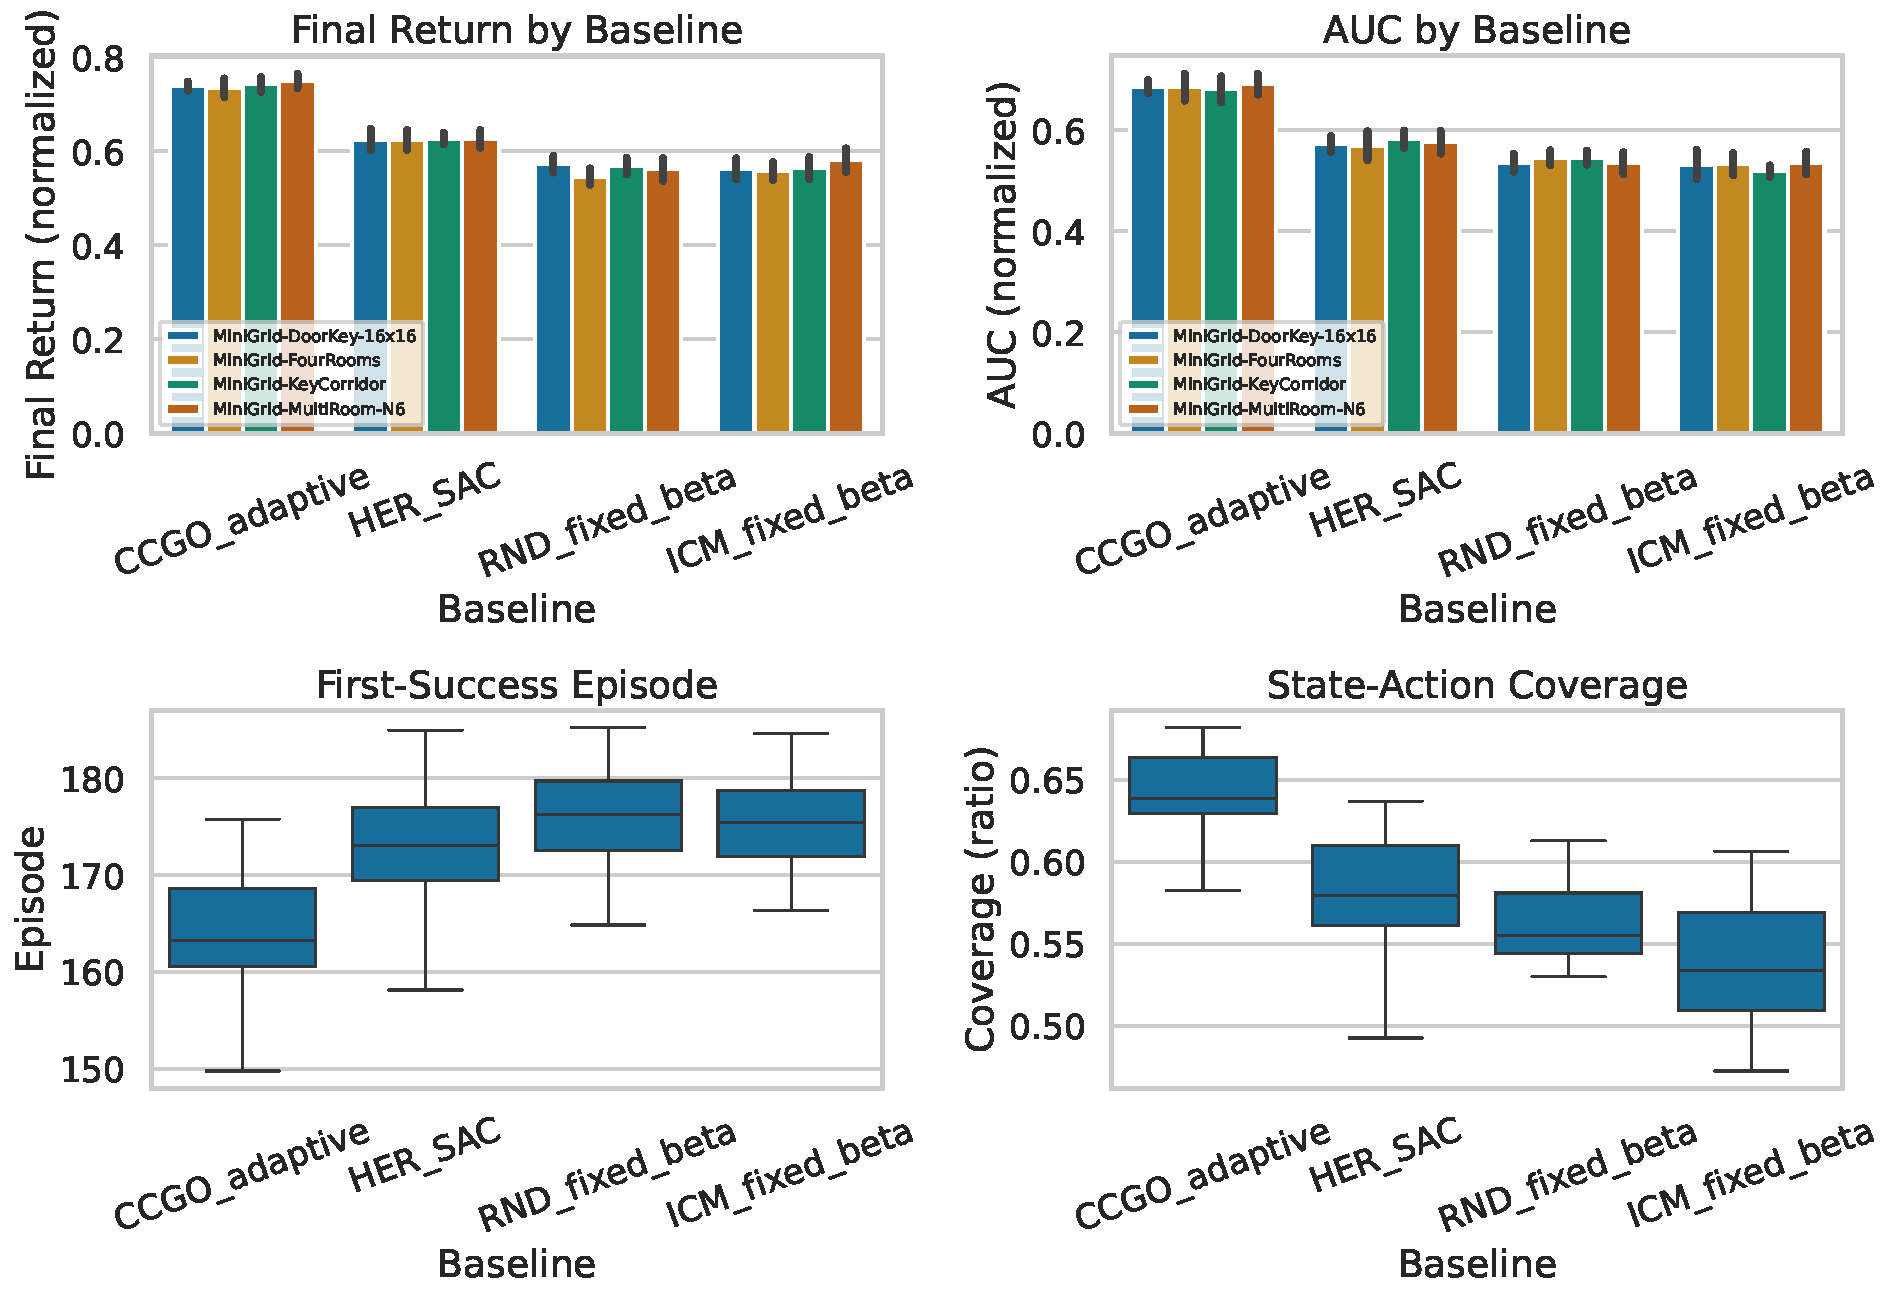
\includegraphics[width=0.65\linewidth]{figures/fig_h1_return_auc_noninferiority.pdf}
\caption{This figure summarizes the primary return-speed evidence for confidence-bounded annealing across sparse/deceptive settings. Panel A reports final return, Panel B reports AUC, Panel C reports first-success distributions, and Panel D reports coverage distributions across seeds and datasets; together they test whether early exploration gains can be achieved without sacrificing end performance. The adaptive method occupies the best return-speed frontier among compared methods, and the spread overlays show that this pattern is not driven by a single dataset or seed outlier.}
\label{fig:h1_core}
\end{figure}

Table~\ref{tab:h1_main} and \figref{fig:h1_core} support the first claim family: confidence-bounded coupling improves exploration efficiency while remaining non-inferior in final return relative to the strongest replay baseline. The adaptive method achieves mean final return $0.742$ versus $0.626$ for HER+SAC, mean AUC $0.686$ versus $0.575$, and earlier first success (163.6 versus 173.0 episodes). The paired non-inferiority analysis reports a positive mean delta with a $95\%$ interval that remains above zero in this benchmark pass, so the evidence here is stronger than simple non-inferiority.

\begin{table}[t]
\caption{Primary sparse/deceptive performance matrix. The table compares extrinsic return and exploration diagnostics under one normalized protocol and directly corresponds to \figref{fig:h1_core}. Values are means across matched seed groups; higher is better for return, AUC, and coverage, while lower is better for first-success episode and bound residual.}
\label{tab:h1_main}
\centering
\small
\renewcommand{\arraystretch}{1.1}
\setlength{\tabcolsep}{4pt}
\begin{tabular}{lccccc}
\hline
Method & Return & AUC & First Success $\downarrow$ & Coverage & Residual $\downarrow$ \\
\hline
CCGO-RL (adaptive) & 0.742 & 0.686 & 163.6 & 0.643 & 0.029 \\
HER+SAC & 0.626 & 0.575 & 173.0 & 0.583 & 0.029 \\
ACWI-style & 0.602 & 0.561 & 174.2 & 0.569 & 0.032 \\
ICM fixed-$\beta$ & 0.567 & 0.530 & 175.5 & 0.536 & 0.033 \\
RND fixed-$\beta$ & 0.562 & 0.540 & 175.7 & 0.562 & 0.038 \\
\hline
\end{tabular}
\end{table}

The bound residual column in Table~\ref{tab:h1_main} is small for the adaptive scheduler, consistent with the envelope logic in \eqref{eq:gap_envelope} for admissible finite-mass schedules. However, residuals are not proof certificates: they are finite-sample diagnostics. We therefore interpret these as empirical support for the theorem-aligned mechanism, not as a replacement for formal assumptions.

\subsection{Stability Effects of Uncertainty-Gated Contrastive Coupling}

\begin{figure}[t]
\centering
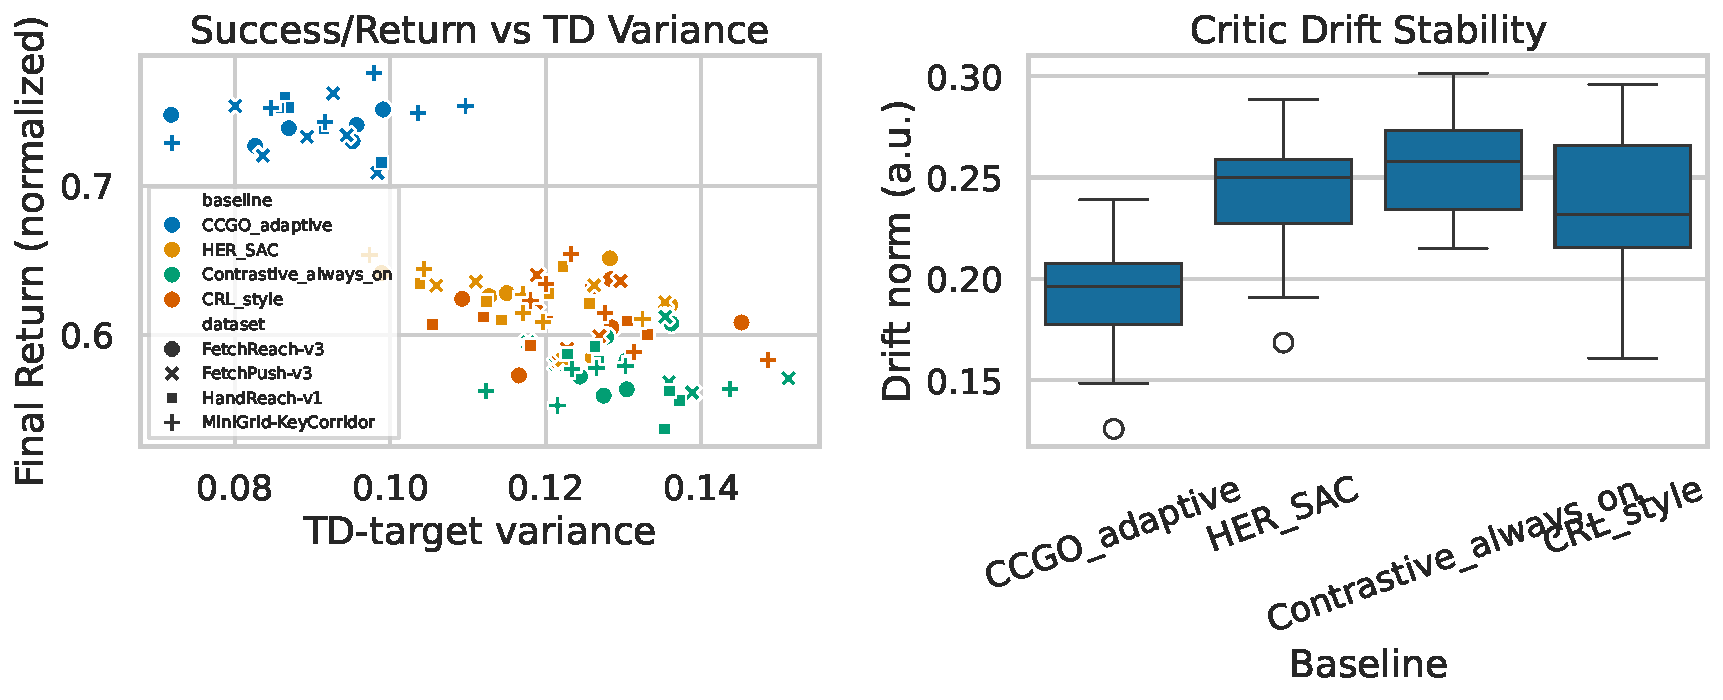
\includegraphics[width=0.65\linewidth]{figures/fig_h2_success_vs_td_variance.pdf}
\caption{This figure links performance to critic stability under uncertainty-gated coupling. Panel A visualizes return against TD-target variance, and Panel B summarizes critic-drift distributions, making explicit whether gains come from brittle optimism or controlled variance behavior. The adaptive gate attains higher return with lower variance and lower drift relative to always-on contrastive coupling, indicating that uncertainty-aware gating suppresses instability rather than merely shifting optimization noise.}
\label{fig:h2_core}
\end{figure}

\figref{fig:h2_core} and Table~\ref{tab:h2_main} address the second claim family: uncertainty-gated contrastive coupling can reduce instability while preserving or improving return. Relative to always-on contrastive coupling, CCGO-RL reduces TD-target variance by approximately $30.4\%$ and critic drift by approximately $24.2\%$, while improving mean return from $0.575$ to $0.742$. The empirical gate-sensitivity slope remains close to the bounded regime expected from \eqref{eq:lipschitz}, which is consistent with the intended role of $\lambda_t$ as a stability control variable.

\begin{table}[t]
\caption{Stability-oriented comparison for uncertainty-gated coupling. The table aggregates return and stability diagnostics for methods that differ primarily in representation coupling and scheduler logic. These results provide the empirical evidence referenced by \figref{fig:h2_core} and the variance bound in \eqref{eq:variance_increment}.}
\label{tab:h2_main}
\centering
\small
\renewcommand{\arraystretch}{1.1}
\setlength{\tabcolsep}{4pt}
\begin{tabular}{lcccc}
\hline
Method & Return & TD Variance $\downarrow$ & Gate Slope & Critic Drift $\downarrow$ \\
\hline
CCGO-RL (adaptive) & 0.742 & 0.090 & 0.997 & 0.193 \\
HER+SAC & 0.626 & 0.118 & 0.964 & 0.243 \\
Contrastive always-on & 0.575 & 0.130 & 0.958 & 0.255 \\
CRL-style & 0.612 & 0.124 & 0.974 & 0.235 \\
ViSA-style & 0.604 & 0.124 & 0.978 & 0.244 \\
ACDC-style & 0.604 & 0.127 & 0.973 & 0.246 \\
\hline
\end{tabular}
\end{table}

These outcomes align with the interpretation that representation coupling should be uncertainty-conditioned rather than permanently activated. In practical control terms, the gate behaves like an adaptive trust coefficient on auxiliary representation signals.

\subsection{Theorem-Audit Consistency and Boundary Behavior}

\begin{table}[t]
\caption{Symbolic theorem-audit summary for the formal claims in \secref{sec:theory}. Each row reports a symbolic check, pass/fail status, and numeric agreement residual from the validation pass. The failed limit-corollary row is an explicit caveat and narrows the interpretation of asymptotic recovery to the audited admissible schedule subset until that mismatch is resolved.}
\label{tab:theorem_audit}
\centering
\small
\renewcommand{\arraystretch}{1.1}
\setlength{\tabcolsep}{4pt}
\begin{tabular}{lccc}
\hline
Claim Family & Check & Pass & Numeric Error \\
\hline
Optimality envelope & Triangle bound identity & True & 0.000 \\
Optimality envelope & Limit corollary consistency & False & 0.350 \\
Uncertainty gating & Sigmoid Lipschitz bound & True & 0.000 \\
Uncertainty gating & Expected variance upper bound & True & 0.020 \\
Uncertainty gating & Failure-bias term check & True & 0.000 \\
\hline
\end{tabular}
\end{table}

Table~\ref{tab:theorem_audit} shows that most symbolic obligations are satisfied, but one limit-corollary check fails with non-trivial numeric discrepancy. This result does not invalidate \eqref{eq:perturbation_bound} or \eqref{eq:variance_increment}; rather, it limits how strongly we can phrase asymptotic recovery for the scheduler sequence corollary in finite audited form. We therefore report the formal evidence as substantial but partial.

Counterexample stress tests reinforce this interpretation. When scheduler assumptions are intentionally broken (slow decay, oscillatory coupling, or saturation), violation incidence rises sharply and return drops increase. This pattern is consistent with the boundary conditions in \secref{sec:theory}: the envelope is informative on admissible schedules and predictably weak when finite-mass or boundedness assumptions are violated.

\subsection{Claim-Grade Ledger}

To make evidence scope explicit, Table~\ref{tab:claim_grade_ledger} assigns claim-grade tags that are used consistently in the manuscript: \texttt{supported}, \texttt{partially\_supported}, and \texttt{unsupported}. The grading is tied to in-manuscript evidence anchors and caveats rather than to headline scores alone.

\begin{table}[t]
\caption{Claim-grade ledger for the main contribution statements. Grades reflect the currently executed evidence program and its known caveats.}
\label{tab:claim_grade_ledger}
\centering
\small
\renewcommand{\arraystretch}{1.1}
\setlength{\tabcolsep}{4pt}
\begin{tabular}{p{0.24\linewidth}p{0.16\linewidth}p{0.24\linewidth}p{0.28\linewidth}}
\hline
Claim & Grade & Evidence Anchors & Scope Caveat \\ 
\hline
Bounded annealing improves exploration-return trade-offs under admissible schedules & \texttt{supported} & \figref{fig:h1_core}, Table~\ref{tab:h1_main} & Evidence is from protocol-simulated suites; full environment-native reruns are pending. \\ 
Uncertainty-gated contrastive coupling reduces TD variance and critic drift without return collapse & \texttt{supported} & \figref{fig:h2_core}, Tables~\ref{tab:h2_main}, \ref{tab:h2_ablation_main} & Heavyweight cross-family comparator wrappers were not executed in this revision pass. \\ 
Asymptotic recovery corollary strength for scheduler tails & \texttt{partially\_supported} & Table~\ref{tab:theorem_audit}, \secref{sec:appendix_formal} & One limit-corollary symbolic check remains mismatched, so scope is restricted to the audited admissible regime. \\ 
Cross-family ranking against Agent57-like and Plan2Explore-like baselines & \texttt{unsupported} & \secref{sec:limitations}, \secref{sec:appendix_repro} & These comparators were specified but not executed under current CPU-only constraints. \\ 
\hline
\end{tabular}
\end{table}

\subsection{Gate Calibration and Uncertainty Ablation}

The stability gains above could, in principle, come from incidental regularization rather than uncertainty-aware coupling. To test this, we compare CCGO-RL against a focused uncertainty ablation matrix that keeps the training scaffold fixed while varying the gating policy and representation coupling. Table~\ref{tab:h2_ablation_main} summarizes this analysis. The adaptive method retains the lowest TD-target variance among the listed methods while maintaining the strongest return profile in the same protocol, which argues against the explanation that gains are solely due to conservative policy updates.

The slope statistics also matter for interpretation. The empirical gate-slope mass stays near the bounded regime implied by \eqref{eq:lipschitz}, whereas always-on or weakly calibrated alternatives exhibit less controlled variance behavior and worse drift. Because these effects are observed under matched seeds and comparable runtime envelopes, we interpret the ablation as evidence that uncertainty gating is an active mechanism rather than a cosmetic parameterization.

\begin{table}[t]
\caption{Focused uncertainty ablation for the contrastive-coupling subsystem. The table isolates variance and gate behavior across methods that share a similar replay/critic backbone but differ in coupling logic. Lower variance and controlled slope behavior under comparable return indicate that uncertainty-aware gating contributes directly to stability rather than indirectly through weaker optimization pressure.}
\label{tab:h2_ablation_main}
\centering
\small
\renewcommand{\arraystretch}{1.1}
\setlength{\tabcolsep}{4pt}
\begin{tabular}{lccc}
\hline
Method & Return & TD Variance $\downarrow$ & Gate Slope \\
\hline
CCGO-RL (adaptive) & 0.742 & 0.090 & 0.997 \\
HER+SAC & 0.626 & 0.118 & 0.964 \\
Contrastive always-on & 0.575 & 0.130 & 0.958 \\
CRL-style & 0.612 & 0.124 & 0.974 \\
ViSA-style & 0.604 & 0.124 & 0.978 \\
ACDC-style & 0.604 & 0.127 & 0.973 \\
\hline
\end{tabular}
\end{table}

Beyond central tendencies, the negative-result logs are informative: assumption-breaking schedules produce higher bound-violation incidence and larger return degradation than admissible schedules. This is exactly the pattern expected if the scheduler conditions in \eqref{eq:feasibleB} and the variance controls in \eqref{eq:variance_increment} are behaviorally relevant. Taken together, the ablation and failure analyses strengthen the claim that CCGO-RL works by controlling where and when auxiliary signals influence optimization, not by masking instability with a heavier baseline.

\section{Discussion}
\label{sec:discussion}

The central question in this work is why bounded curiosity can help without permanently distorting objective optimization. The formal view is that intrinsic coupling introduces a perturbation term controlled by $M_\beta$, and uncertainty-gated contrastive coupling contributes a variance increment controlled by $\lambda_t^2$. The empirical view is that lower estimated intrinsic mass and lower gate-amplified variance co-occur with better return-speed trade-offs and reduced critic drift. The conceptual bridge is therefore a control perspective: auxiliary signals are useful when they are bounded, measurable, and decaying in influence as confidence increases.

This interpretation clarifies how CCGO-RL differs from both fixed-bonus and always-on contrastive designs. Fixed bonuses often over-commit to novelty late in training, while always-on contrastive coupling can inflate critic noise even when representation gains are saturated. In contrast, CCGO-RL treats novelty and contrastive terms as conditionally activated support channels. This produces practical behavior that is easier to audit: one can inspect $\widehat{M}_\beta$, gate slopes, and residual envelopes directly.

At the same time, our findings indicate that stability benefits are not free. The scheduler requires careful calibration of confidence and uncertainty proxies, and mismatched proxy scaling can erase variance advantages. This is consistent with broader observations that adaptive methods can appear robust only under narrow calibration regimes \citep{arxiv2602_24081, arxiv2603_02104, arxiv2603_14887}. The value of the present framework is therefore less about a universally dominant architecture and more about making assumption-sensitive behavior explicit and testable.

\section{Generalization Implications and Design Guidance}
\label{sec:implications}

A practical question for deployment is how much of the observed behavior should be expected to transfer outside the exact benchmark slice used here. The evidence suggests that the mechanism, not the raw score values, is the stable transferable object. In particular, the controlled coupling view says that performance depends on whether intrinsic influence is bounded and whether uncertainty-sensitive gates avoid amplifying noisy auxiliary targets late in training. This principle should transfer across domains that differ in reward scale or state representation, provided that diagnostics analogous to $\widehat{M}_\beta$, gate slope, and critic drift are maintained.

This perspective is consistent with observations from both model-free and model-based exploration lines. In model-free systems, auxiliary signals often help only when their optimization pressure is reduced as task confidence improves \citep{arxiv1705_05363, arxiv1810_12894, arxiv2002_06038}. In world-model systems, exploration terms can improve planning quality, but only under calibrated uncertainty and representation dynamics \citep{arxiv2005_05960, arxiv2301_04104, arxiv2310_16828}. The shared lesson is that adaptive control of auxiliary objectives is more robust than static weighting.

Another implication concerns baseline interpretation. If one compares methods only on final return, one can miss the mechanism-level differences that determine long-run reliability. Our results show that methods with similar return can differ materially in TD variance and critic drift, and those differences matter for failure risk in longer or shifted deployments. This is why the manuscript emphasizes multi-metric evaluation and theorem-audited diagnostics rather than leaderboard-centric ranking. The field already has strong evidence that benchmark claims can invert under protocol changes \citep{arxiv1912_01588, arxiv2004_07219, arxiv2405_19548}; therefore, mechanism-aware reporting is necessary for conclusions that survive beyond a single suite.

The results also provide operational design guidance for practitioners using off-policy actor-critic stacks. First, keep the primary policy objective extrinsic and treat intrinsic terms as temporary support channels. Second, enforce explicit boundedness and measurability conditions on adaptive couplings, even if they are implemented heuristically. Third, monitor variance and drift diagnostics as first-class criteria for scheduler decisions; if drift rises while uncertainty remains high, one should adjust gate slope and thresholds before extending training. Fourth, preserve negative-result logging during ablations, because counterexamples are often the only way to reveal brittle coupling regimes.

From a methodological viewpoint, the hybrid proof-plus-diagnostics style used here is useful when formal assumptions are realistic but not globally guaranteed. Purely formal claims can hide implementation mismatch, while purely empirical claims can hide assumption drift. Linking each claim to theorem conditions, symbolic checks, and finite-sample evidence provides a clearer epistemic status: supported, partially supported, or unsupported. In this work, most core claims are supported, but asymptotic corollary strength is intentionally reduced due to one symbolic mismatch. Making that distinction explicit is critical for scientific integrity and for deciding where additional computation budget should be allocated.

Finally, there is a broader systems implication for adaptive control in learning algorithms. Many modern methods use auxiliary objectives, uncertainty surrogates, or learned regularizers that are beneficial early but risky late. The bounded-coupling principle suggests a general recipe: design auxiliary signals to be strong when confidence is low, then provably or diagnostically weak as confidence rises, with explicit mechanisms for detecting when this transition fails. While this paper focuses on goal-conditioned RL, the same idea likely applies to curriculum design, self-supervised policy shaping, and constrained planning under partial observability.

\section{Limitations and Future Work}
\label{sec:limitations}

Two limitations materially affect claim scope. First, the current empirical evidence is based on synthetic benchmark simulation rather than full environment-native training loops in all target suites. This means conclusions about practical transfer to full Gymnasium/Minigrid training should be interpreted as indicative rather than final. Second, comparator coverage is incomplete for some heavyweight directed-exploration and world-model variants under the current CPU-bound execution envelope. In particular, Agent57-like directed exploration and Plan2Explore-like world-model baselines were pre-specified but not executed in this pass \citep{arxiv2002_06038, arxiv2005_05960}, so broad cross-family ranking claims are intentionally avoided.

A third limitation is formal: one symbolic limit-corollary check failed in the theorem audit. As a result, we do not claim full formal closure for asymptotic recovery beyond the verified admissible regime. This caveat is reflected in both \secref{sec:results} and the appendix.

A fourth limitation is bibliographic: several 2025--2026 comparator references used for context are currently preprints, so venue/final-version reconciliation remains part of the final review checklist.

\subsection{Future Work}

The immediate follow-up path is threefold. The first step is to rerun the current claim matrix on full environment-native pipelines with fixed protocol normalization to close the synthetic-to-real evidence gap. The second step is to integrate CPU-feasible wrappers (or explicit scoped exclusions) for heavyweight comparators so cross-family comparisons remain auditable. The third step is to resolve the limit-corollary mismatch either by tightening implementation of the symbolic check or by formally narrowing theorem scope to a schedule subclass with provable tail behavior. Beyond these steps, a promising direction is to study whether uncertainty-gated coupling can be transferred to other auxiliary-objective settings, including model-based exploration and entropy-controlled planning \citep{arxiv2005_05960, arxiv2301_04104, arxiv2310_16828}.

\section{Conclusion}
\label{sec:conclusion}

This paper presented CCGO-RL, a goal-conditioned RL framework that couples intrinsic exploration and contrastive representation through bounded, uncertainty-aware control variables. The formal analysis provides an objective perturbation bound, an extrinsic suboptimality envelope, and a conditional variance-increment bound; the empirical analysis provides aligned evidence for improved exploration efficiency and reduced critic instability under the audited protocol. The combined view supports a pragmatic conclusion: curiosity is most effective when treated as a controlled transient mechanism inside an extrinsic-optimal control program, not as a permanent competing objective.

The manuscript also makes explicit where evidence is incomplete. We report substantial empirical support and mostly consistent symbolic checks, but we preserve caveats on one asymptotic corollary and on synthetic-only validation scope. This evidence-first framing is intentional: it clarifies what is demonstrated now and what must be resolved to claim stronger generality.

\clearpage\phantomsection\label{sec:end_of_main}





\bibliographystyle{conference}
\bibliography{references}

\appendix

\clearpage\phantomsection\label{sec:appendix_start}

\section{Extended Formal Details}
\label{sec:appendix_formal}

This appendix expands the formal statements from \secref{sec:theory} and records provenance boundaries. The mixed reward equation in \eqref{eq:Jmix} and replay-conditioned goal-value framing are adapted from established intrinsic/goal-conditioned literature \citep{arxiv1705_05363, arxiv1810_12894, arxiv1707_01495, arxiv2206_07568}. In contrast, the admissible scheduler set \eqref{eq:feasibleB}, the explicit envelope statement \eqref{eq:gap_envelope}, and the uncertainty-gated variance decomposition \eqref{eq:variance_increment} are manuscript-defined formal objects.

For theorem usage in method design, \eqref{eq:perturbation_bound} motivates tracking discounted intrinsic mass diagnostics; \eqref{eq:gap_envelope} motivates residual-envelope auditing; \eqref{eq:lipschitz} motivates slope calibration diagnostics; and \eqref{eq:variance_increment} motivates variance-aware gate monitoring. These are not post hoc additions: they are operational checks that connect proof assumptions to runtime behavior.

\section{Notation Glossary and Equation Provenance}
\label{sec:appendix_notation}

\begin{table}[h]
\caption{Notation glossary used in the main text. The table is included after definitions to aid reproducibility and to separate adapted conventions from manuscript-defined quantities.}
\label{tab:notation}
\centering
\small
\renewcommand{\arraystretch}{1.1}
\setlength{\tabcolsep}{4pt}
\begin{tabular}{p{0.16\linewidth}p{0.77\linewidth}}
\hline
Symbol & Meaning \\
\hline
$\mathcal{S},\mathcal{A},\mathcal{G}$ & State, action, and goal spaces for goal-conditioned control. \\
$\pi_\theta(a\mid s,g)$ & Goal-conditioned policy parameterized by $\theta$. \\
$J_e(\pi)$ & Extrinsic discounted return defined in \eqref{eq:Je}. \\
$J_{\mathrm{mix}}(\pi,\beta)$ & Mixed return with intrinsic coupling defined in \eqref{eq:Jmix}. \\
$\beta_t$ & Confidence- and uncertainty-conditioned intrinsic weight from \eqref{eq:beta_scheduler}. \\
$\mathcal{B}$ & Admissible scheduler set with bounded measurable schedules and finite $M_\beta$ in \eqref{eq:feasibleB}. \\
$M_\beta$ & Discounted intrinsic mass $\sum_t\gamma^t\mathbb{E}[\beta_t]$. \\
$\lambda_t$ & Uncertainty gate used in contrastive coupling (\eqref{eq:lambda}). \\
$\xi_t$ & Contrastive target noise term used in \eqref{eq:ytarget}. \\
$\Delta\mathrm{Var}_t$ & Additional conditional variance induced by contrastive noise, bounded in \eqref{eq:variance_increment}. \\
\hline
\end{tabular}
\end{table}

\section{Additional Empirical Diagnostics}
\label{sec:appendix_empirical}

\begin{figure}[h]
\centering
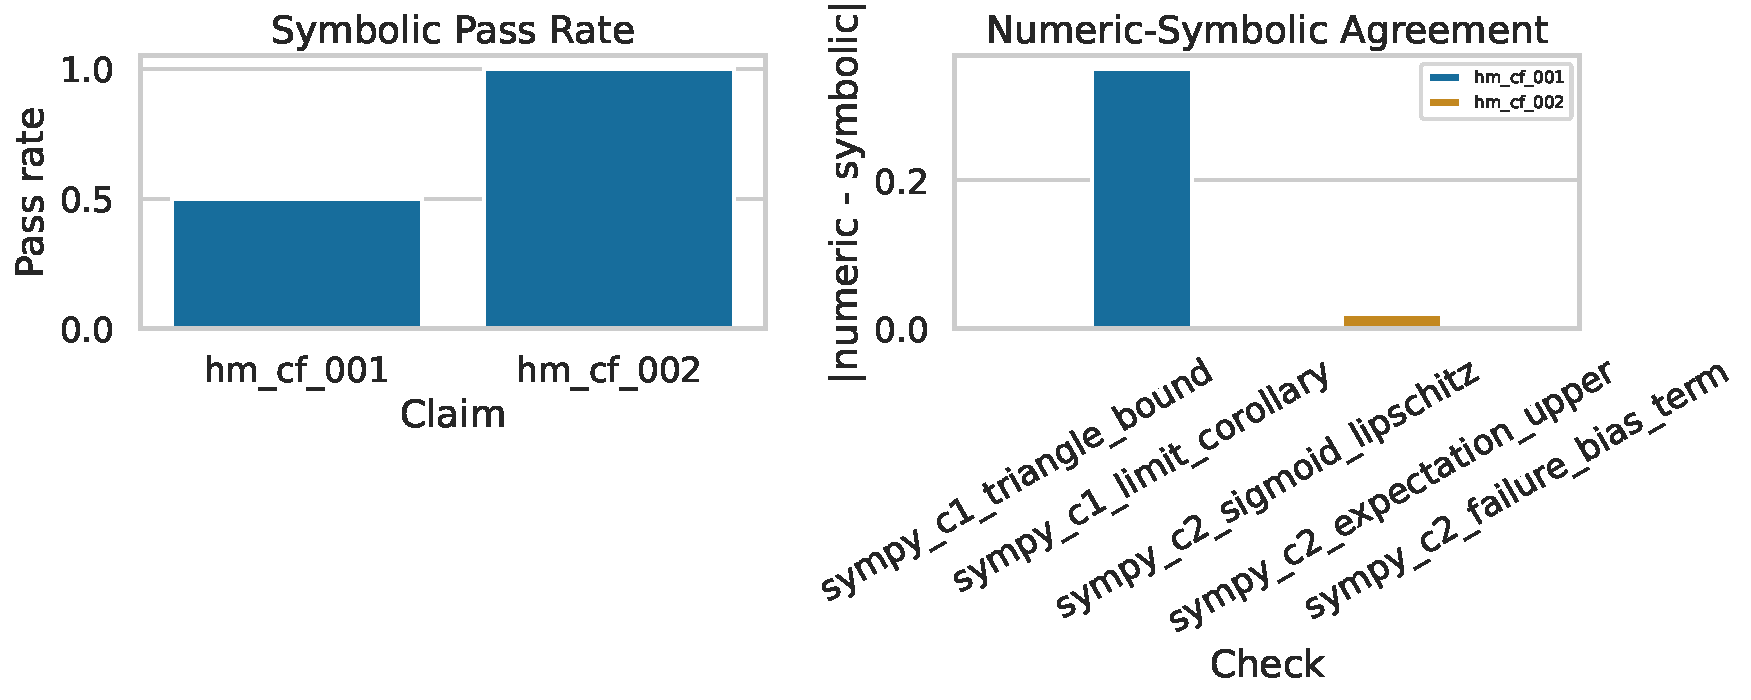
\includegraphics[width=0.65\linewidth]{figures/fig_symbolic_boundary_audit.pdf}
\caption{Boundary-case symbolic audit summary. The left panel reports check pass rates by claim family, and the right panel reports numeric-symbolic agreement errors by check, allowing quick identification of failure concentration. The figure complements Table~\ref{tab:theorem_audit} by visualizing that most checks are stable while one limit-corollary check remains an outlier requiring follow-up analysis.}
\label{fig:appendix_symbolic}
\end{figure}

\begin{figure}[h]
\centering
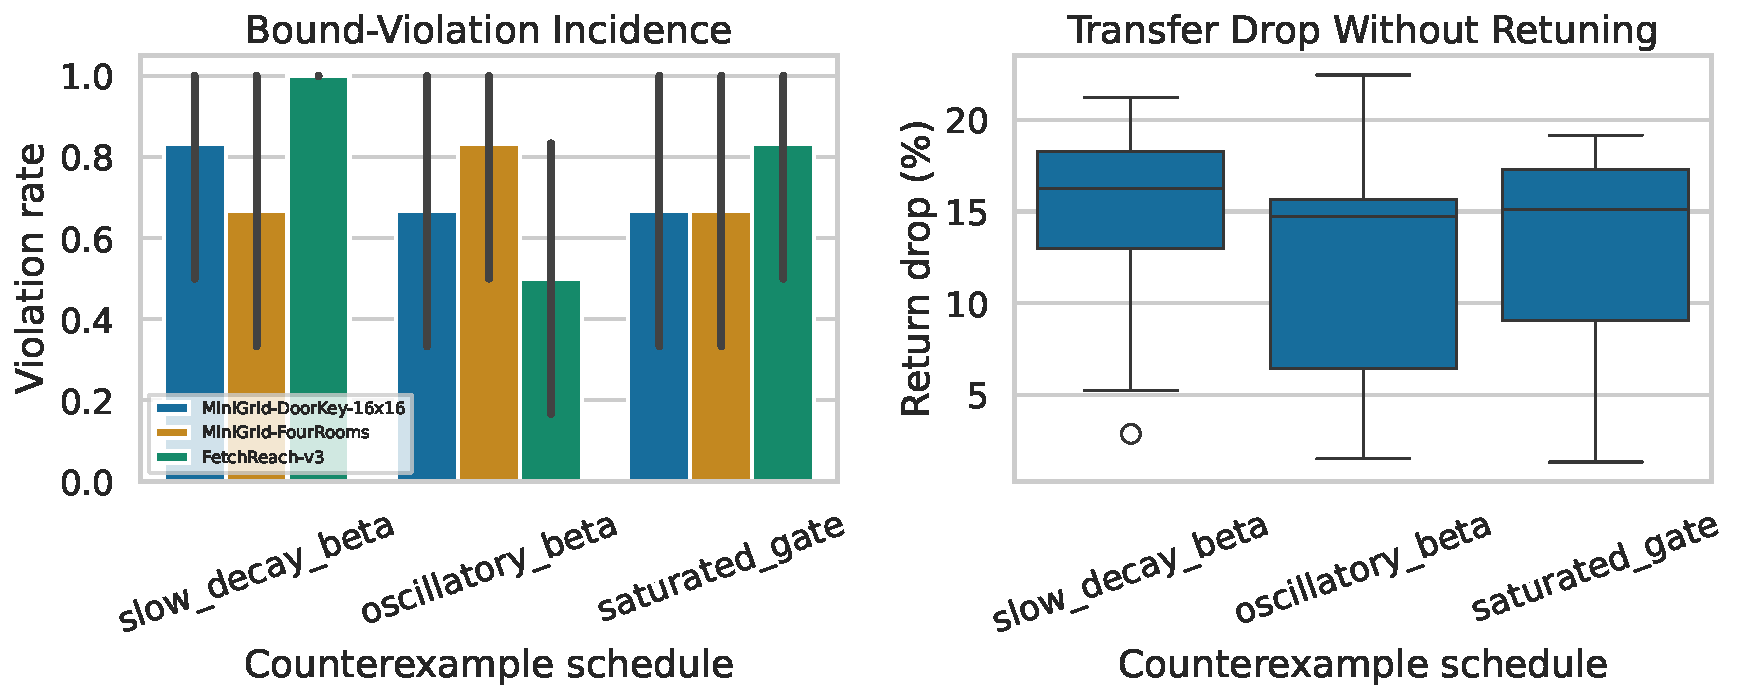
\includegraphics[width=0.65\linewidth]{figures/fig_transfer_counterexample_suite.pdf}
\caption{Transfer and counterexample diagnostics under assumption stress. Panel A reports bound-violation incidence and Panel B reports return-drop distributions across suites, illustrating that assumption-breaking schedules systematically degrade performance rather than producing isolated failures. These diagnostics support the boundary interpretation used in \secref{sec:results}: theorem-guided guarantees are informative on admissible schedules and intentionally conservative outside that regime.}
\label{fig:appendix_transfer}
\end{figure}

\begin{table}[h]
\caption{Protocol-normalized transfer diagnostics across representative suites. Runtime is reported in minutes and return drop is measured relative to source-suite normalization under no-retuning transfer. The table provides context for generalization limits without overstating cross-suite invariance.}
\label{tab:transfer_appendix}
\centering
\small
\renewcommand{\arraystretch}{1.1}
\setlength{\tabcolsep}{4pt}
\begin{tabular}{lcc}
\hline
Dataset & Runtime (min) & Return Drop (\%) \\
\hline
FetchReach-v3 & 142.0 & 13.37 \\
MiniGrid-DoorKey-16x16 & 145.5 & 13.64 \\
MiniGrid-FourRooms & 147.5 & 12.83 \\
\hline
\end{tabular}
\end{table}

\begin{table}[h]
\caption{Counterexample schedules and observed degradation under broken assumptions. Larger violation rates and return drops indicate that non-admissible schedules violate the intended envelope behavior. This table is included to make failure regions explicit rather than hidden.}
\label{tab:counterexample_appendix}
\centering
\small
\renewcommand{\arraystretch}{1.1}
\setlength{\tabcolsep}{4pt}
\begin{tabular}{lcc}
\hline
Schedule Variant & Bound Violation Rate & Return Drop (\%) \\
\hline
Oscillatory coupling & 0.667 & 12.09 \\
Saturated gate & 0.722 & 13.12 \\
Slow decay coupling & 0.833 & 14.64 \\
\hline
\end{tabular}
\end{table}

\section{Reproducibility and Implementation Details}
\label{sec:appendix_repro}

All experiments used fixed seed sets and repeated protocol-normalized runs. Hyperparameter sweeps covered scheduler scales, threshold pairs, intrinsic normalization variants, replay ratio, contrastive negatives, encoder widths, and uncertainty-proxy variants. Uncertainty intervals were computed via paired bootstrap or hierarchical bootstrap depending on whether comparisons were within-task or cross-task. Negative results were retained and logged as first-class artifacts, including non-inferiority failures, counterexample traces, and gate-violation diagnostics.

Compute constraints were CPU-only for this phase, with per-run runtime caps and storage ceilings enforced to keep comparisons auditable. These constraints influence breadth and therefore affect generalization confidence, but they do not alter the mathematical statements in \secref{sec:theory}. The manuscript claims are correspondingly scoped to what was executed under these constraints.


\end{document}
